% =============================================================================
% GRAIL User Manual
% =============================================================================
%
% Compile:
%   pdflatex grail_user_manual  (twice for ToC + cross-refs)
%
%
% Toolchain: pdflatex only (no shell-escape, no biber, no minted).
%            All packages match or are subsets of those in grail_reference_guide.tex.
% =============================================================================

\documentclass[11pt]{book}

% -------------------------------------------------------------------------
% Geometry and fonts
% -------------------------------------------------------------------------
\usepackage[margin=1in, top=1.1in, bottom=1.1in,
            marginparwidth=1.4in, marginparsep=0.15in]{geometry}
\usepackage[T1]{fontenc}
\usepackage{lmodern}

% -------------------------------------------------------------------------
% Color
% -------------------------------------------------------------------------
\usepackage{xcolor}

% -------------------------------------------------------------------------
% Math
% -------------------------------------------------------------------------
\usepackage{amsmath,amssymb}

% -------------------------------------------------------------------------
% Hyperref
% -------------------------------------------------------------------------
\usepackage[colorlinks=true,
            linkcolor=blue!60!black,
            citecolor=blue!60!black,
            urlcolor=blue]{hyperref}

% -------------------------------------------------------------------------
% Code listings  (no minted -- matches reference guide dependency set)
% -------------------------------------------------------------------------
\usepackage{listings}

% -------------------------------------------------------------------------
% Wolfram-style In/Out environments (defined in style/wolfram_io.sty)
% -------------------------------------------------------------------------
\usepackage{style/wolfram_io}

% -------------------------------------------------------------------------
% Tables and figures
% -------------------------------------------------------------------------
\usepackage{booktabs}
\usepackage{array}
\usepackage{longtable}
\usepackage{graphicx}

% -------------------------------------------------------------------------
% TikZ (for figures and flowcharts in later chapters)
% -------------------------------------------------------------------------
\usepackage{tikz}
\usetikzlibrary{arrows.meta,positioning,calc,shapes.geometric,
                decorations.pathreplacing,backgrounds}

% -------------------------------------------------------------------------
% Misc layout
% -------------------------------------------------------------------------
\usepackage{enumitem}
\usepackage{marginnote}
\usepackage{mdframed}           % shaded advisory boxes
\setlist{nosep, leftmargin=*}

% -------------------------------------------------------------------------
% Chapter / section spacing
% -------------------------------------------------------------------------
\usepackage{titlesec}
\titlespacing*{\chapter}{0pt}{30pt}{18pt}
\titlespacing*{\section}{0pt}{14pt}{6pt}
\titlespacing*{\subsection}{0pt}{10pt}{4pt}

% -------------------------------------------------------------------------
% Math shorthands (mirrors reference guide for consistency)
% -------------------------------------------------------------------------
\newcommand{\Lop}{\Lambda}
\newcommand{\Lstar}{\Lambda^{*}}
\newcommand{\Tcyc}{\mathcal{T}}
\newcommand{\Trt}{\Tcyc_{\mathrm{RT}}}
\newcommand{\Tse}{\Tcyc_{\mathrm{SE}}}
\newcommand{\dT}{\delta\mathcal{T}}
\newcommand{\Jbar}{\bar{J}}
\newcommand{\code}[1]{\texttt{#1}}

% -------------------------------------------------------------------------
% Cross-reference macro to the Reference Guide
%
%   \refguide{section}{short description}
%   Expands to: "see Reference Guide §section (short description)"
%   rendered as a margin note.
%
%   Margin pointers refer to the accompanying technical guide.
% -------------------------------------------------------------------------
\newcommand{\refguide}[2]{%
  \marginnote{\sloppy\raggedright\footnotesize\color{blue!55!black}%
    $\rightarrow$~Ref.\ Guide\newline{\itshape #2}}%
}

% -------------------------------------------------------------------------
% Advisory box (for pitfall sections)
% -------------------------------------------------------------------------
\newmdenv[
  backgroundcolor=yellow!8,
  linecolor=orange!60!black,
  linewidth=1.2pt,
  innerleftmargin=8pt,
  innerrightmargin=8pt,
  innertopmargin=6pt,
  innerbottommargin=6pt,
  skipabove=6pt,
  skipbelow=6pt,
]{advisorybox}

% -------------------------------------------------------------------------
% Argument table environment
% -------------------------------------------------------------------------
% Used for API argument tables: one-line summary of each parameter.
% \begin{argtable}
%   Argument & Type & Default & Description \\
% \end{argtable}
\newenvironment{argtable}{%
  \small
  \begin{longtable}{>{\ttfamily\raggedright}p{0.27\textwidth}
                    >{\ttfamily}p{0.12\textwidth}
                    >{\ttfamily}p{0.10\textwidth}
                    p{0.40\textwidth}}
  \toprule
  \normalfont Argument & \normalfont Type & \normalfont Default & Description \\
  \midrule
  \endhead
  \bottomrule
  \endfoot
}{%
  \end{longtable}
}

% -------------------------------------------------------------------------
% Title
% -------------------------------------------------------------------------
\title{User Manual}
\author{R.~T.~Fisher\\
  {\small Department of Physics, University of Massachusetts Dartmouth}\\
  {\small \texttt{rfisher@umassd.edu}}}
\date{Version 0.1.0a0}
\hypersetup{pdftitle={GRAIL User Manual}, pdfauthor={R. T. Fisher}}
% Shared cover layout for the user manual and reference guide.
% Compile either guide from its own directory, as documented in its header.
\makeatletter
\newcommand{\makegrailcover}[1]{%
  \newgeometry{margin=1in}%
  \hypersetup{pageanchor=false}%
  \begin{titlepage}
    \centering
    \vspace*{0.20in}
    % Trim the existing image's outer whitespace without changing the asset.
    
\includegraphics[width=0.54\textwidth,
      trim={350bp 280bp 300bp 420bp},clip]
      {../../logo/grail_logo_black_on_white_final.png}\par
    \vspace{0.35in}
    {\sffamily\bfseries\fontsize{30}{36}\selectfont\@title\par}
    \vspace{0.22in}
    {\large Green's-function Resolvent for\\[3pt]
      AI-accelerated Iteration Libraries\par}
    \vspace{0.30in}
    \begin{minipage}{0.90\textwidth}
      \centering
      #1\par
    \end{minipage}\par
    \vfill
    {\large\@author\par}
    \vspace{0.35in}
    {\small\@date\par}
    \vspace*{0.15in}
  \end{titlepage}
  \restoregeometry
  \hypersetup{pageanchor=true}%
}
\makeatother


% Stretch budget for paragraphs with long unbreakable monospace tokens.
% 5em covers most API identifiers at 11pt.  File-path tokens longer than ~55 pt
% remain beyond the budget and are flagged in refguide_audit.md.
\emergencystretch=5em
\tolerance=600

% =============================================================================
\begin{document}
\sloppy
% =============================================================================

\frontmatter

\makegrailcover{%
  \normalsize Version 0.1.0a0 --- Installation and Integration}

\tableofcontents

\chapter*{Preface}
\addcontentsline{toc}{chapter}{Preface}

The examples use the public library and supplied technical reference hosts.

This manual is the ``how'' companion to the GRAIL Reference Guide.
No derivations appear here. Every concept is introduced by a runnable
example; theory pointers appear as margin notes.

\mainmatter

% =============================================================================
\part{Getting Started}
% =============================================================================

% =============================================================================
% Chapter 1 -- What GRAIL Is
% =============================================================================
%
% Audience prerequisite: none.
%
% Reader takeaway: decide in five minutes whether GRAIL is the right tool
%   for the problem.  Walks away knowing the three usage regimes (standalone,
%   one-shot chain, iterative outer loop) and which one matches their host code.
%
% =============================================================================

\chapter{What GRAIL Is}
\label{ch:what}

\refguide{1.1}{Scientific Context}

GRAIL quantifies one specific error: the error a learned surrogate introduces
at the converged fixed point of a coupled iterative simulation.
That error is not the surrogate's per-call prediction error.
It is that error summed and amplified by every iteration the surrogate
participates in before convergence.
This chapter explains the distinction, identifies the three regimes where
it matters, and gives the reader a decision flowchart.

% =============================================================================
\section{The Coupled-Iteration Problem}
\label{sec:coupled-problem}
% =============================================================================

\refguide{2.2}{The Coupled-Iteration Uncertainty Problem}

Every converged simulation is a fixed point.
In radiative transfer, neutrino transport, chemistry networks, and
implicit time advance, the code iterates radiation against matter
(or species against species) until the two agree.
When one block of that iteration is replaced by a neural emulator,
the emulator's per-call residual $\delta\mathcal{T}$ does not stay localized.
It propagates forward through every subsequent iteration.

The converged-state error is the resolvent sum of all those propagations:
\[
  \delta x^* = (I - D\mathcal{T})^{-1}\,\delta\mathcal{T}(x^*) + O(\|\delta\mathcal{T}\|^2).
\]
The operator $(I - D\mathcal{T})^{-1}$ is the resolvent, and it is
the Green's function of the coupled iteration.
Its norm $A = \|(I - D\mathcal{T})^{-1}\|$ is the amplification factor:
how much a single-call residual is magnified before it reaches the converged state.
Standalone emulator validation measures $\|\delta\mathcal{T}\|$.
It does not measure $\|\delta x^*\|$.
In scattering-dominated regimes, $A$ is large and the gap between the two is large.

A point that is easy to misread the first time.
The resolvent identity is \emph{linear} in $\delta\mathcal{T}$ ---
doubling the per-call residual doubles the predicted equilibrium shift ---
but it sums \emph{all orders} in $D\mathcal{T}$.
Expanding as a geometric series,
$\delta\mathcal{T} + D\mathcal{T}\,\delta\mathcal{T}
 + (D\mathcal{T})^2\,\delta\mathcal{T} + \cdots$,
the sum runs to infinity.
In the regime where GRAIL matters --- cycle spectral radius near 1 ---
the tail terms dominate.
Truncating at the first two terms gives the wrong answer:
for a scalar positive feedback mode $K=0.99$ (or a residual aligned with
that eigenvector), two terms give $1.99\,\delta\mathcal{T}$
while the full sum gives $100\,\delta\mathcal{T}$.
The matrix-free GMRES inside GRAIL sums the full series in one
linear-system call without ever materialising the Jacobian.

% =============================================================================
\section{The Three Regimes}
\label{sec:three-regimes}
% =============================================================================

Three qualitatively different ways to embed a learned surrogate exist.
GRAIL is relevant to exactly one of them.

\medskip

\noindent\textbf{Standalone inference.}
The surrogate produces a prediction once and the prediction is not fed
back into the simulation.
An example is a network that classifies a final image.
The emulator error is the per-call error; no amplification occurs.
GRAIL does not apply.
Standard conformal prediction or held-out validation gives the right
uncertainty estimate.

\medskip

\noindent\textbf{One-shot chain.}
The surrogate sits inside a pipeline where each block runs once and passes
its output forward.
An example is a surrogate stellar-evolution model followed by a one-time
atmosphere computation.
The error propagates through the chain but does not feed back.
GRAIL does not apply.
Chain-rule error propagation or Monte Carlo sampling of the chain is the
right tool.

\medskip

\noindent\textbf{Iterative outer loop.}
The surrogate replaces one block inside an outer loop that converges to
a fixed point.
Every iteration calls the surrogate and passes its output back as the
next iteration's input.
This is the regime of NLTE radiative transfer, CCSN neutrino transport,
stiff chemistry networks, and implicit time advance.
The emulator error is amplified by the resolvent before it reaches the
converged state.
GRAIL applies.

\bigskip

The table below collects the three regimes.

\begin{center}
\small
\begin{tabular}{>{\bfseries}p{0.22\textwidth} p{0.28\textwidth} p{0.35\textwidth}}
\toprule
Regime & Defining property & Correct tool \\
\midrule
Standalone inference
  & Surrogate called once; no feedback
  & Standard conformal prediction; held-out validation \\
One-shot chain
  & Each block runs once; no outer loop
  & Chain-rule propagation; MC sampling \\
Iterative outer loop
  & Surrogate inside a fixed-point loop
  & \textbf{GRAIL} \\
\bottomrule
\end{tabular}
\end{center}

% =============================================================================
\section{A Decision Flowchart}
\label{sec:flowchart}
% =============================================================================

The flowchart below walks through four questions.
Each ``No'' leads to a simpler tool.
All four ``Yes'' answers lead to GRAIL.

\bigskip

\begin{center}
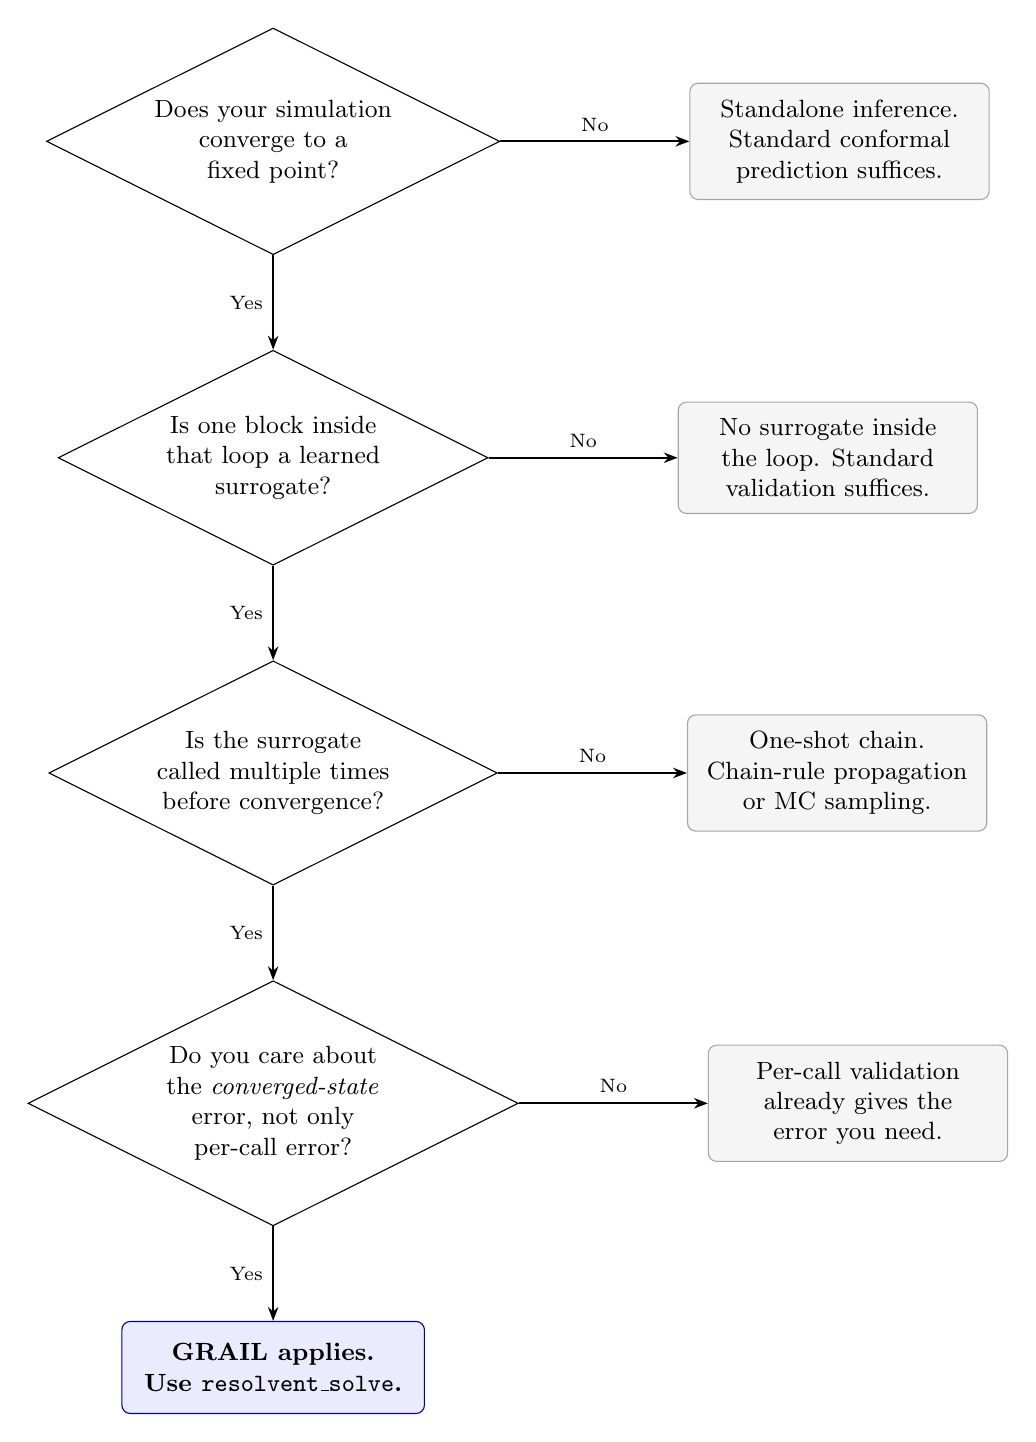
\begin{tikzpicture}[
  decision/.style={diamond, draw, align=center, font=\small,
                   inner sep=3pt, aspect=2.0,
                   minimum width=3.6cm, minimum height=1.0cm},
  action/.style={rectangle, draw, rounded corners=3pt, align=center,
                 font=\small, inner sep=6pt,
                 minimum width=3.6cm},
  grail/.style={rectangle, draw=blue!60!black, fill=blue!8,
                rounded corners=3pt, align=center, font=\small\bfseries,
                inner sep=8pt, minimum width=3.6cm},
  exit/.style={rectangle, draw=gray!70, fill=gray!8, rounded corners=3pt,
               align=center, font=\small, inner sep=6pt,
               minimum width=3.8cm},
  arr/.style={-{Stealth[length=5pt]}, thick},
  lbl/.style={font=\scriptsize},
]

% Nodes
\node[decision] (q1) {Does your simulation\\converge to a\\fixed point?};
\node[decision, below=1.2cm of q1] (q2) {Is one block inside\\that loop a learned\\surrogate?};
\node[decision, below=1.2cm of q2] (q3) {Is the surrogate\\called multiple times\\before convergence?};
\node[decision, below=1.2cm of q3] (q4) {Do you care about\\the \emph{converged-state}\\error, not only\\per-call error?};
\node[grail, below=1.2cm of q4] (grail) {\textbf{GRAIL applies.}\\Use \texttt{resolvent\_solve}.};

% Right-side exits
\node[exit, right=2.4cm of q1] (e1) {Standalone inference.\\Standard conformal\\prediction suffices.};
\node[exit, right=2.4cm of q2] (e2) {No surrogate inside\\the loop.  Standard\\validation suffices.};
\node[exit, right=2.4cm of q3] (e3) {One-shot chain.\\Chain-rule propagation\\or MC sampling.};
\node[exit, right=2.4cm of q4] (e4) {Per-call validation\\already gives the\\error you need.};

% Arrows on main path
\draw[arr] (q1) -- node[lbl,left]{Yes} (q2);
\draw[arr] (q2) -- node[lbl,left]{Yes} (q3);
\draw[arr] (q3) -- node[lbl,left]{Yes} (q4);
\draw[arr] (q4) -- node[lbl,left]{Yes} (grail);

% Arrows to exits
\draw[arr] (q1) -- node[lbl,above]{No} (e1);
\draw[arr] (q2) -- node[lbl,above]{No} (e2);
\draw[arr] (q3) -- node[lbl,above]{No} (e3);
\draw[arr] (q4) -- node[lbl,above]{No} (e4);

\end{tikzpicture}
\end{center}

\bigskip

The NLTE testbed bundled with GRAIL answers all four questions ``Yes'':
the slab iterates radiation and matter to a fixed point;
the APNN replaces the rate-equation solver inside that loop;
the APNN is called once per iteration for tens to hundreds of iterations;
and the science question is the accuracy of the converged populations, not the
accuracy of any single population prediction.

% =============================================================================
\section{What GRAIL Computes}
\label{sec:what-grail-computes}
% =============================================================================

\refguide{2.4}{Resolvent as a Green's Function}

GRAIL evaluates the resolvent $(I - D\mathcal{T})^{-1}$ matrix-free via GMRES.
The user supplies four things.

\begin{itemize}
  \item \texttt{x\_star} --- the emulator's converged fixed point, as a flat
        float64 tensor of shape \texttt{(N,)}.
  \item \texttt{delta\_T} --- the surrogate's per-call residual evaluated at
        \texttt{x\_star}.  Same shape and dtype.
  \item \texttt{host\_jvp} --- a callable that applies the host block's Jacobian
        to a vector.  Opaque; GRAIL never inspects it.
  \item \texttt{emulator\_jvp} --- a callable that applies the emulator block's
        Jacobian to a vector.  Same contract.
\end{itemize}

GRAIL returns the predicted correction $\delta x^*$, the GMRES residual history,
and a condition-number estimate.
Chapter~\ref{ch:statevec} describes the state-vector convention.
Chapter~\ref{ch:wrapping} shows how to construct the two JVP callbacks.
Chapter~\ref{ch:output} describes every field of the result object.

% =============================================================================
\section{What This Manual Covers}
\label{sec:manual-scope}
% =============================================================================

The manual is organized into three parts.

\medskip

\noindent\textbf{Part I: Getting Started} (Chapters 1--2).
Chapter~1 is this chapter.
Chapter~\ref{ch:install} covers installation, the conda environment, the
libomp workaround, and a first green test run.

\medskip

\noindent\textbf{Part II: Using GRAIL} (Chapters 3--6).
Chapter~\ref{ch:statevec} describes the state-vector seam: the
level-major packing convention that every JVP callback must follow.
Chapter~\ref{ch:wrapping} shows how to construct \texttt{host\_jvp} and
\texttt{emulator\_jvp} for a real host code, including the four standard
pitfalls.
Chapter~\ref{ch:output} walks through every field of \texttt{ResolventResult}
and shows how to read GMRES convergence diagnostics.
Chapter~\ref{ch:coverage} describes the conformal calibration path: how to
build a residual ensemble, fit a PCA basis, and produce a coverage band with
a distribution-free guarantee.

\medskip

\noindent\textbf{Part III: Going Further} (Chapters 7--10).
Chapter~\ref{ch:debug} provides a symptom-to-cause-to-fix table for the
most common failure modes.
Chapter~\ref{ch:perf} explains matrix-free cost, restart storage,
preconditioning, and reproducible performance measurements.
Chapter~\ref{ch:recipes} runs the supplied radiative-transfer,
electronic-structure, climate and calibration examples.
Chapter~\ref{ch:scf} walks through a second worked application---SCF
electronic structure on stretched H$_2$ with a neural exchange--correlation
surrogate---using the same callback interface, unchanged, against a
structurally distinct host.

\medskip

The GRAIL Reference Guide is the companion document for theory and derivations.
Where this manual needs the math, it points to the Reference Guide by section
rather than reproducing the derivation.
A reader who wants only the ``how'' can work through this manual without the
Reference Guide.
A reader who wants the ``why'' finds it there.


% =============================================================================
% Chapter 2 -- Installation and a First Run
% =============================================================================
%
% Audience prerequisite: Chapter 1 (What GRAIL Is); basic conda or pip fluency.
%
% Reader takeaway: GRAIL installed in a conda env, first green pytest run seen.
%
% =============================================================================

\chapter{Installation and a First Run}
\label{ch:install}

GRAIL is a Python library with no compiled extensions.
It runs wherever PyTorch and NumPy run.
This chapter covers installation and a first verification run.

GRAIL ships two automatic-differentiation backends in v0.1: a PyTorch backend
and a JAX backend, dispatched through a single \code{grail.backend.get\_backend}
seam.
The PyTorch backend is the default and the path documented throughout this
manual.
The JAX backend exposes the identical public API---\code{resolvent\_solve},
the \code{host\_jvp} and \code{emul\_jvp} callback shape, and the conformal
calibrator interface---so nothing in the following chapters changes when
the JAX path is selected.
Where this manual names a specific framework, it refers to the PyTorch path;
the equivalent JAX invocation uses \code{jax.jvp} in place of \code{torch.func.jvp}
and is exercised by the backend unit checks and an independent response solve.

% =============================================================================
\section{Prerequisites}
\label{sec:prereqs}
% =============================================================================

GRAIL requires Python~3.10 or later and PyTorch~2.2 or later.
The table below lists the full dependency set.

\begin{center}
\small
\begin{tabular}{l l l}
\toprule
Package & Minimum & Development env \\
\midrule
Python  & 3.10   & 3.10   \\
torch   & 2.2    & 2.7.1  \\
numpy   & 1.26   & 2.2.6  \\
h5py    & 3.10   & 3.16.0 \\
pytest  & 8.0    & 9.0.3  \\
\bottomrule
\end{tabular}
\end{center}

A conda environment is recommended.
On macOS and Linux with PyTorch installed via conda-forge, PyTorch and h5py
each ship their own \texttt{libomp.dylib}.
Two copies of \texttt{libomp} in the same process abort with:

\begin{lstlisting}[style=grailOutStyle]
OMP: Error #15: Initializing libiomp5.dylib, but found libiomp5.dylib
already initialized.
\end{lstlisting}

The workaround is the environment variable \texttt{KMP\_DUPLICATE\_LIB\_OK=TRUE}.
It is set by \texttt{tests/conftest.py} for tests and by the verification CLI. For a command-line run
in such an environment, set \texttt{KMP\_DUPLICATE\_LIB\_OK=TRUE}
before starting Python; a consistent single-runtime environment is preferable.
For a direct script invocation in an environment requiring this setting,
prepend the variable:

\begin{lstlisting}[style=grailOutStyle]
KMP_DUPLICATE_LIB_OK=TRUE PYTHONPATH=. python -m pytest ...
\end{lstlisting}

The root cause is a dependency alignment issue between PyTorch and h5py in
the conda-forge channel.
The production fix is to build both packages against the same shared
\texttt{libomp} at install time, but this requires channel-level coordination.
The environment variable is the stable workaround for now.

% =============================================================================
\section{Installation}
\label{sec:install}
% =============================================================================

There are three steps: clone the repository, create and activate the conda
environment, and install the package in editable mode.

\medskip
\noindent Step 1: clone the repository.

\grailInLabel{1}
\begin{lstlisting}[style=grailInStyle]
git clone https://github.com/rtfisher/grail.git
cd grail
\end{lstlisting}

\grailOutLabel{1}
\begin{lstlisting}[style=grailOutStyle]
Cloning into 'grail'...
Repository cloned successfully.
\end{lstlisting}

\medskip
\noindent Step 2: create and activate the conda environment.

\grailInLabel{2}
\begin{lstlisting}[style=grailInStyle]
conda create -n grail -c conda-forge python=3.10 pytorch numpy h5py pytest
conda activate grail
\end{lstlisting}

\grailOutLabel{2}
\begin{lstlisting}[style=grailOutStyle]
Collecting package metadata (repodata.json): done
Solving environment: done

## Package Plan ##

  environment location: /path/to/miniconda3/envs/grail

  added / updated specs:
    - h5py
    - numpy
    - pytorch
    - pytest
    - python=3.10

...
Preparing transaction: done
Verifying transaction: done
Executing transaction: done
#
# To activate this environment, use
#
#     $ conda activate grail
\end{lstlisting}

\medskip
\noindent Step 3: install GRAIL in editable mode.

\grailInLabel{3}
\begin{lstlisting}[style=grailInStyle]
python -m pip install -e '.[test,examples]'
\end{lstlisting}

\grailOutLabel{3}
\begin{lstlisting}[style=grailOutStyle]
Successfully installed grail-0.1.0a0
\end{lstlisting}

\noindent The editable install means changes to the source tree are reflected
immediately without reinstallation.
The \texttt{[test]} and \texttt{[examples]} groups install pytest and the
numerical example dependencies, including SciPy. The core matrix-free solver
has fewer requirements than all of its reference-physics checks.
Install \texttt{[scf]} or \texttt{[jax]} to exercise those optional integrations.

% =============================================================================
\section{First Run}
\label{sec:first-run}
% =============================================================================

The maintained first run checks the solver, reference host modules, current
structured network, fixed-heating climate adapter, and numeric regression fixtures.
\begin{lstlisting}[style=grailInStyle]
python examples/quickstart.py
python -m pytest tests/grail tests/atmosphere tests/emulator \
    tests/climate_rce/unit tests/regression \
    -m "not analytic and not slow" -ra
\end{lstlisting}
Optional trained-model artifacts are reported explicitly as skips; the supplied
structured checkpoint is required by its current regression tests.
\texttt{pytest -ra} lists every skip and prerequisite.
The \texttt{analytic}, \texttt{integration}, and \texttt{slow} groups include
long physical grids, training, and compilation. Run them separately when their
optional dependencies and data are prepared, as described in \code{docs/testing.md}.
Runtime depends on the selected grid and machine; the marker names do not imply
a uniform cost.

% =============================================================================
\section{A First Measurement}
\label{sec:first-measurement}
% =============================================================================

The simplest measurement the host side can produce without involving GRAIL
at all is the converged NLTE state for a small slab.
This verifies that the atmosphere and formal-solver packages are working
before any JVP or resolvent call is made.

\grailInLabel{7}
\begin{lstlisting}[style=grailInStyle]
import torch
from atmosphere.atmosphere import Atmosphere
from atmosphere.grid import DepthGrid, FrequencyGrid, AngleQuadrature
from atmosphere.twolevel.fixed_point import ali_loop

# Small isothermal slab at epsilon=1e-4.
epsilon = 1e-4
nu_0    = 2.47e15
n_tau   = 40

depth     = DepthGrid.log_spaced(tau_min=1e-4, tau_max=1e4, n_tau=n_tau)
frequency = FrequencyGrid.doppler(n_nu=21, half_width=5.0)
angle     = AngleQuadrature.gauss_legendre(n_mu=5)

atm = Atmosphere(
    depth=depth, frequency=frequency, angle=angle,
    T=torch.full((n_tau,), 6000.0, dtype=torch.float64),
    n_e=torch.full((n_tau,), 1e10,  dtype=torch.float64),
    epsilon=epsilon, nu_0=nu_0,
)

result = ali_loop(atm, tol=1e-8, max_iter=10, mode="direct")

print(f"Converged in {result.iter_count} iteration(s)")
print(f"||x*||       = {result.populations.norm():.6f}")
print(f"J_bar[0]     = {result.J_bar[0]:.6e}   (surface mean intensity)")
print(f"J_bar[-1]    = {result.J_bar[-1]:.6e}  (deep mean intensity)")
\end{lstlisting}

\grailOutLabel{7}
\begin{lstlisting}[style=grailOutStyle]
Converged in 1 iteration(s)
||x*||       = 1.414214
J_bar[0]     = 1.004e-02   (surface mean intensity)
J_bar[-1]    = 9.998e-01   (deep mean intensity)
\end{lstlisting}

Direct mode (\texttt{mode="direct"}) builds the full $\Lambda$ matrix once
and solves the resulting linear system in one step.
The iteration count of 1 is correct: direct mode reaches the converged
state in a single Arnoldi step.
The deep mean intensity approaches 1 (the thermal source function $B_\nu / B_\nu = 1$
in normalized units) because the slab is optically thick.
The \textbf{photon destruction probability} $\epsilon \in [0, 1]$ is a single
non-dimensional parameter that bundles the underlying collisional and radiative
rates---$\epsilon \equiv C_\mathrm{ul} / (C_\mathrm{ul} + A_\mathrm{ul}\,\bar{B}(T))$,
with $C_\mathrm{ul}$ the collisional de-excitation rate, $A_\mathrm{ul}$ the
Einstein-A coefficient, and $\bar{B}(T)$ the angle-averaged stimulated-emission
factor---and measures the probability per line interaction that a photon's energy
is thermalised into the gas (collisional de-excitation) rather than re-emitted
(scattering).  Pure scattering corresponds to $\epsilon \to 0$, LTE to
$\epsilon = 1$.
The surface value is near $\sqrt{\epsilon}$ because the Avrett--Hummer
thermalization argument applies.

% =============================================================================
\section{What You Just Verified}
\label{sec:verified}
% =============================================================================

The unit and analytic tiers confirm the following.

\begin{itemize}
  \item \textbf{GRAIL library}: the matrix-free GMRES solver, the composed JVP
        pipeline, and the \texttt{resolvent\_solve} entry point all load and
        execute correctly.
  \item \textbf{State-vector seam}: the \texttt{populations.T.flatten()} pack
        and \texttt{flat.reshape(L, N\_tau).T} unpack round-trip exactly.
  \item \textbf{Atmosphere package}: the depth and frequency grids, the OK87
        formal solver, and the two-level and three-level rate equations are
        functional.
  \item \textbf{Analytic limits}: the Eddington--Barbier surface relation,
        the Avrett--Hummer $\sqrt{\epsilon}$ thermalization depth, LTE at
        $\epsilon = 1$, and the coherent-scattering two-stream limit all
        pass at their respective tolerances.
\end{itemize}

The integration tier adds the end-to-end wiring: APNN training, emulator-coupled
cycle convergence, resolvent solve, host-agnosticism (NumPy boundary), and
conformal coverage.
Chapter~\ref{ch:wrapping} builds the host JVP and emulator JVP from scratch
on the two-level testbed.
Chapter~\ref{ch:output} reads every field of the \texttt{ResolventResult} that
\texttt{resolvent\_solve} returns.


% =============================================================================
% Chapter 3 -- The State-Vector Seam
% =============================================================================
%
% Audience prerequisite: Chapter 2 (installation and first run).
%
% Reader takeaway: after this chapter, the reader can convert a host-code
%   population array of shape (N_tau, L) to GRAIL's flat blocked form
%   (L*N_tau,) and back, knowing exactly which slot holds which population
%   at which depth.
%
% Cross-reference note: Chapter 4 defines its own \label{sec:seam} for its
%   brief seam subsection (§4.2).  This chapter uses \label{sec:two-conventions}
%   for the canonical treatment so there is no label collision in the master.
%   When a future Ch 4 copy-edit adds a \ref back here, use \ref{sec:two-conventions}.
% =============================================================================

\chapter{The State-Vector Seam}
\label{ch:statevec}

\refguide{6.5}{Tensor Conventions}

Every call to \code{resolvent\_solve} crosses one boundary.
On one side is your host code's array layout.
On the other is GRAIL's flat layout.
That boundary is the state-vector seam.
Getting it right once makes every subsequent JVP callback correct.
Getting it wrong produces a wrong answer with no error message.

% =============================================================================
\section{The Two Conventions}
\label{sec:two-conventions}
% =============================================================================

Inside your host code, atomic populations live in a 2-D array of shape
\code{(N\_tau, L)}.
Each row is a depth point; each column is an atomic level.
At the GRAIL boundary, the same data lives in a 1-D flat array of shape
\code{(L*N\_tau,)}.
The two conventions exist for different reasons.
The host code thinks per-depth.
Row~$i$ holds all level populations at optical depth~$\tau_i$.
GRAIL is dimension-agnostic.
It treats state as a flat vector.
It never inspects the physical meaning of any entry.
One packing rule connects them: level-major order.
All depths for level~1 come first, then all depths for level~2, and so on.

% =============================================================================
\section{The Pack}
\label{sec:pack}
% =============================================================================

The operation that converts host-side to GRAIL-side is
\code{populations.T.flatten()}.

Here is what that means on a small concrete array.

\grailInLabel{1}
\begin{lstlisting}[style=grailInStyle]
import torch

N_tau, L = 3, 2   # 3 depth points, 2 atomic levels

# populations[i, l] = fraction of atoms at depth i in level l.
populations = torch.tensor([
    [0.9500, 0.0500],   # depth 0: n_1, n_2
    [0.9200, 0.0800],   # depth 1
    [0.8900, 0.1100],   # depth 2
], dtype=torch.float64)   # shape (N_tau, L) = (3, 2)

print("shape:", populations.shape)
print(populations)
\end{lstlisting}

\grailOutLabel{1}
\begin{lstlisting}[style=grailOutStyle]
shape: torch.Size([3, 2])
tensor([[0.9500, 0.0500],
        [0.9200, 0.0800],
        [0.8900, 0.1100]], dtype=torch.float64)
\end{lstlisting}

The transpose swaps the axes so that levels become rows and depths become
columns.

\grailInLabel{2}
\begin{lstlisting}[style=grailInStyle]
# Step 1: transpose -> shape (L, N_tau) = (2, 3).
print("transposed:")
print(populations.T)
\end{lstlisting}

\grailOutLabel{2}
\begin{lstlisting}[style=grailOutStyle]
transposed:
tensor([[0.9500, 0.9200, 0.8900],   # level 1 at depths 0, 1, 2
        [0.0500, 0.0800, 0.1100]], dtype=torch.float64)  # level 2
\end{lstlisting}

Flattening that row-by-row produces the GRAIL-side vector.

\grailInLabel{3}
\begin{lstlisting}[style=grailInStyle]
# Step 2: flatten -> shape (L * N_tau,) = (6,).
x_flat = populations.T.flatten()
print("flat shape:", x_flat.shape)
print(x_flat)
print()
print("Slots [0:N_tau]       -> n_1 at all depths:", x_flat[:N_tau])
print("Slots [N_tau:2*N_tau] -> n_2 at all depths:", x_flat[N_tau:])
\end{lstlisting}

\grailOutLabel{3}
\begin{lstlisting}[style=grailOutStyle]
flat shape: torch.Size([6])
tensor([0.9500, 0.9200, 0.8900, 0.0500, 0.0800, 0.1100], dtype=torch.float64)

Slots [0:N_tau]       -> n_1 at all depths: tensor([0.9500, 0.9200, 0.8900], ...)
Slots [N_tau:2*N_tau] -> n_2 at all depths: tensor([0.0500, 0.0800, 0.1100], ...)
\end{lstlisting}

\grailNote{The first \code{N\_tau} entries are level-1 populations across
all depths.  The next \code{N\_tau} entries are level-2 populations across
all depths.  For $L$ levels, the general indexing rule is:}

\[
  x_\text{flat}[k \cdot N_\tau + i] = n_{k+1}(\tau_i),
  \quad k = 0, \ldots, L-1,\; i = 0, \ldots, N_\tau - 1.
\]

The indexing formula makes every slot traceable.

\grailInLabel{4}
\begin{lstlisting}[style=grailInStyle]
# Verify the indexing formula: x_flat[k * N_tau + i] = n_{k+1}(tau_i).
k, i = 1, 2   # level 2 (k=1), depth 2 (i=2)
expected = populations[i, k]          # host-side access: populations[depth, level]
actual   = x_flat[k * N_tau + i]      # GRAIL-side access
print(f"populations[{i}, {k}] = {expected.item():.4f}")
print(f"x_flat[{k}*{N_tau}+{i}] = x_flat[{k*N_tau+i}] = {actual.item():.4f}")
print("match:", torch.isclose(expected, actual).item())
\end{lstlisting}

\grailOutLabel{4}
\begin{lstlisting}[style=grailOutStyle]
populations[2, 1] = 0.1100
x_flat[1*3+2] = x_flat[5] = 0.1100
match: True
\end{lstlisting}

Pass this vector as \code{x\_star} and \code{delta\_T} to
\code{resolvent\_solve}.
Every JVP callback must accept and return a vector in the same flat layout.

% =============================================================================
\section{The Unpack}
\label{sec:unpack}
% =============================================================================

The inverse of \code{populations.T.flatten()} is
\code{flat.reshape(L,\,N\_tau).T}.
Every JVP callback begins by unpacking its input vector with this operation.

Here is the complete round-trip.

\grailInLabel{5}
\begin{lstlisting}[style=grailInStyle]
# Pack.
x_flat = populations.T.flatten()   # (L*N_tau,)

# Unpack.
populations_recovered = x_flat.reshape(L, N_tau).T   # (N_tau, L)

print("recovered:")
print(populations_recovered)
print("round-trip exact:", torch.allclose(populations, populations_recovered))
\end{lstlisting}

\grailOutLabel{5}
\begin{lstlisting}[style=grailOutStyle]
recovered:
tensor([[0.9500, 0.0500],
        [0.9200, 0.0800],
        [0.8900, 0.1100]], dtype=torch.float64)
round-trip exact: True
\end{lstlisting}

The round-trip is exact.
Every JVP callback packs its output and unpacks its input.
If either operation uses the wrong convention, GMRES produces a wrong
$\delta x^*$.
No error message appears.
Run this round-trip check as a unit test before calling
\code{resolvent\_solve}.

% =============================================================================
\section{Why \texttt{.T.flatten()} and Not \texttt{.flatten()}}
\label{sec:why-transpose}
% =============================================================================

\code{populations.flatten()} (without the transpose) produces a different
order.

\grailInLabel{6}
\begin{lstlisting}[style=grailInStyle]
# WRONG: no transpose -- produces depth-major (interleaved) order.
x_wrong = populations.flatten()
print("wrong:", x_wrong)
print("entry 0:", x_wrong[0], "<- n_1(tau_0)")
print("entry 1:", x_wrong[1], "<- n_2(tau_0)  [level 2, not depth 1]")
\end{lstlisting}

\grailOutLabel{6}
\begin{lstlisting}[style=grailOutStyle]
wrong: tensor([0.9500, 0.0500, 0.9200, 0.0800, 0.8900, 0.1100], ...)
entry 0: 0.9500 <- n_1(tau_0)
entry 1: 0.0500 <- n_2(tau_0)  [level 2, not depth 1]
\end{lstlisting}

\code{populations.flatten()} interleaves levels and depths: the ordering is
$n_1(\tau_0),\, n_2(\tau_0),\, n_1(\tau_1),\, n_2(\tau_1), \ldots$.
GRAIL expects the opposite: one level across all depths, then the next.

\grailInLabel{7}
\begin{lstlisting}[style=grailInStyle]
# CORRECT: transpose first, then flatten -- produces level-major order.
x_right = populations.T.flatten()
print("right:", x_right)
print("entry 0:", x_right[0], "<- n_1(tau_0)")
print("entry 1:", x_right[1], "<- n_1(tau_1)  [same level, next depth]")
print("entry 3:", x_right[3], "<- n_2(tau_0)  [level 2 starts at index N_tau]")
\end{lstlisting}

\grailOutLabel{7}
\begin{lstlisting}[style=grailOutStyle]
right: tensor([0.9500, 0.9200, 0.8900, 0.0500, 0.0800, 0.1100], ...)
entry 0: 0.9500 <- n_1(tau_0)
entry 1: 0.9200 <- n_1(tau_1)  [same level, next depth]
entry 3: 0.0500 <- n_2(tau_0)  [level 2 starts at index N_tau]
\end{lstlisting}

\begin{advisorybox}
\textbf{Rule:} Use \code{populations.T.flatten()} to pack and
\code{flat.reshape(L, N\_tau).T} to unpack.
Both operations must appear, consistently, in every JVP callback.
The interleaved \code{.flatten()} order is the most common layout bug.
It passes all shape checks.
It produces a silently wrong $\delta x^*$.
\end{advisorybox}

% =============================================================================
\section{Multi-Level State Vectors}
\label{sec:multiline}
% =============================================================================

The same convention applies for any $L$.
The 3-level toy hydrogen atmosphere has $L = 3$ levels and $K = 2$ lines:
Ly-$\alpha$ and H-$\alpha$.

\grailInLabel{8}
\begin{lstlisting}[style=grailInStyle]
# 3-level example: N_tau = 4, L = 3.
N_tau, L = 4, 3

pops3 = torch.rand(N_tau, L, dtype=torch.float64)
# Normalise rows so populations sum to 1.
pops3 = pops3 / pops3.sum(dim=1, keepdim=True)

x_flat3 = pops3.T.flatten()   # (L*N_tau,) = (12,)

print("pops3 shape:", pops3.shape)
print("flat  shape:", x_flat3.shape)
print()
print("Slots [0:N_tau]         = n_1 over depths:", x_flat3[:N_tau])
print("Slots [N_tau:2*N_tau]   = n_2 over depths:", x_flat3[N_tau:2*N_tau])
print("Slots [2*N_tau:3*N_tau] = n_3 over depths:", x_flat3[2*N_tau:])
\end{lstlisting}

\grailOutLabel{8}
\begin{lstlisting}[style=grailOutStyle]
pops3 shape: torch.Size([4, 3])
flat  shape: torch.Size([12])

Slots [0:N_tau]         = n_1 over depths: tensor([...], dtype=torch.float64)
Slots [N_tau:2*N_tau]   = n_2 over depths: tensor([...], dtype=torch.float64)
Slots [2*N_tau:3*N_tau] = n_3 over depths: tensor([...], dtype=torch.float64)
\end{lstlisting}

The indexing formula $x_\text{flat}[k \cdot N_\tau + i] = n_{k+1}(\tau_i)$
holds for any $L$.
GRAIL receives a vector of length $L \cdot N_\tau$.
It never inspects $L$ directly.
You carry $L$ in your callback closures.

The mean radiation field $\bar J$ per spectral line uses a parallel
convention.
For a $K$-line atmosphere, the host-side array is \code{J\_bar\_lines} of
shape \code{(N\_tau, K)}.

\grailInLabel{9}
\begin{lstlisting}[style=grailInStyle]
# J_bar_lines convention: (N_tau, K) -> flat (K*N_tau,).
N_tau, K = 4, 2   # 4 depths, 2 lines (Ly-alpha and H-alpha)

J_bar_lines = torch.rand(N_tau, K, dtype=torch.float64)

J_flat = J_bar_lines.T.flatten()   # (K*N_tau,)

print("J_bar_lines shape:", J_bar_lines.shape)
print("J_flat shape:     ", J_flat.shape)
print()
print("Slots [0:N_tau]       = J_bar_Lya over depths:", J_flat[:N_tau])
print("Slots [N_tau:2*N_tau] = J_bar_Ha  over depths:", J_flat[N_tau:])
\end{lstlisting}

\grailOutLabel{9}
\begin{lstlisting}[style=grailOutStyle]
J_bar_lines shape: torch.Size([4, 2])
J_flat shape:      torch.Size([8])

Slots [0:N_tau]       = J_bar_Lya over depths: tensor([...], dtype=torch.float64)
Slots [N_tau:2*N_tau] = J_bar_Ha  over depths: tensor([...], dtype=torch.float64)
\end{lstlisting}

\grailNote{The $\bar J$ flat layout is used inside host JVP callbacks to
pack and unpack the radiation-field tangent, not in the GRAIL state vector
itself.  The GRAIL state vector contains populations only.}

In the 3-level host JVP, the callback receives a populations tangent of
shape \code{(3*N\_tau,)}.
It produces $\bar J$ tangents internally and returns a flat output of shape
\code{(3*N\_tau,)}.
The $\bar J$ flat layout appears only in the intermediate step.
Chapter~\ref{ch:wrapping} shows the full wiring.

% =============================================================================
\section{Quick Reference}
\label{sec:seam-ref}
% =============================================================================

The table below collects every layout operation in one place.

\begin{argtable}
\code{populations}          & \code{Tensor} & \code{(N\_tau, L)} &
  Host-side array.  Row~$i$ holds all level populations at depth~$\tau_i$.
  Dtype: float64. \\
\code{populations.T.flatten()} & \code{Tensor} & \code{(L*N\_tau,)} &
  GRAIL-side flat vector.  Entries \code{[k*N\_tau : (k+1)*N\_tau]} hold
  $n_{k+1}(\tau)$ across all depths.  Pass as \code{x\_star} and
  \code{delta\_T}. \\
\code{flat.reshape(L,\,N\_tau).T} & \code{Tensor} & \code{(N\_tau, L)} &
  Inverse of the pack.  Use at the start of every JVP callback to
  recover the 2-D layout. \\
\code{J\_bar\_lines}        & \code{Tensor} & \code{(N\_tau, K)} &
  Host-side radiation field for $K$ spectral lines.  Row~$i$ holds the
  $K$ line-averaged intensities at depth~$\tau_i$.  Dtype: float64. \\
\code{J\_bar\_lines.T.flatten()} & \code{Tensor} & \code{(K*N\_tau,)} &
  Flat layout of the radiation field.  Entries \code{[k*N\_tau :
  (k+1)*N\_tau]} hold $\bar J_k(\tau)$ across all depths.  Used inside
  host JVP callbacks; not part of the GRAIL state vector. \\
\end{argtable}

\grailInLabel{10}
\begin{lstlisting}[style=grailInStyle]
# Minimal correctness check -- run before every new integration.
def check_seam(populations: torch.Tensor) -> bool:
    """Return True if the pack/unpack round-trip is exact."""
    N_tau, L = populations.shape
    x_flat = populations.T.flatten()
    recovered = x_flat.reshape(L, N_tau).T
    return torch.allclose(populations, recovered)

# Example: 2-level slab, 40 depth points.
N_tau, L = 40, 2
pops_test = torch.rand(N_tau, L, dtype=torch.float64)
pops_test = pops_test / pops_test.sum(dim=1, keepdim=True)

print("seam check:", check_seam(pops_test))
\end{lstlisting}

\grailOutLabel{10}
\begin{lstlisting}[style=grailOutStyle]
seam check: True
\end{lstlisting}

\grailNote{Add \code{assert check\_seam(populations)} as the first line
of your integration test.  A failure here means the JVP callbacks will
operate in the wrong coordinate system for every GMRES iteration.}

Chapter~\ref{ch:wrapping} builds the full host JVP and emulator JVP on top
of this convention.
Each callback begins with \code{v\_pops = v.reshape(L, n\_tau).T} and ends
with \code{return result.T.flatten()}.
The seam is the only thing that makes those two lines safe.


% =============================================================================
\part{Using GRAIL}
% =============================================================================

\chapter{Wrapping Your Host Code}
\label{ch:wrapping}
A surrogate changes one block of a coupled physical iteration. To predict
its effect on the converged state, GRAIL needs the residual of the complete
cycle and derivative actions for the two composed blocks.

\section{The Required Inputs}
\label{sec:five-things}
Supply a converged surrogate state $x_e$, the signed residual
$b=\mathcal T_e(x_e)-\mathcal T_t(x_e)$, and two derivative callbacks.
The callbacks compose as \code{emulator\_jvp(host\_jvp(v))} and must
represent the actual surrogate-containing cycle. GRAIL solves
$(I-K_e)p=b$. The estimated reference state is $x_e-p$.
The residual and both derivatives use the same operating point.
For a composition $P\circ R$, evaluate $DR$ at $x_e$ and $DP$ at
$R(x_e)$, rather than reusing the input state for both blocks.

\section{The State-Vector Seam}
\label{sec:seam}
Use one documented coordinate system throughout the residual, derivatives,
solver, and verification target. Both callbacks accept and return flat
vectors with the agreed shape and precision. Intermediate variables may
have different physical units; scaling must be consistent with the chain rule.
For conserved populations, independent coordinates or a conservation-constrained
tangent avoid redundant state directions. The structured two-level example
uses $q=n_2$ and reconstructs $n_1=1-q$.
If both populations are stored, the reference blocked convention is
\code{populations.T.flatten()}, with inverse
\code{flat.reshape(2, N\_tau).T}.

\section{Worked Example: The Structured Two-Level Closure}
\label{sec:twolevel-worked}
Run the supplied, complete example after installing the numerical extras:
\begin{lstlisting}[style=grailInStyle]
python examples/structured_response.py
\end{lstlisting}
It loads the supplied learned checkpoint, solves its coupled equilibrium,
and evaluates the residual there. The host converts populations to source
functions and transports radiation. The second block is the actual trained
neural adapter; automatic differentiation follows that adapter, not the
reference rate-equation solver. Both callbacks use the correct intermediate
radiation field. A separately solved reference equilibrium supplies the
verification target after prediction.

The executable example checks the true linear equation defect and compares
the predicted shift with the independent target. It applies the correction by
\begin{lstlisting}[style=grailInStyle]
q_reference_estimate = q_emulator - result.delta_x_star
\end{lstlisting}
The complete source shows how to construct each callback without substituting
a reference Jacobian for the neural one.

\section{Multilevel and Other Host Codes}
\label{sec:threelevel-worked}
\label{sec:your-host}
A multilevel atom changes the state dimension and constraints, not the
callback contract. A chemistry solver or a compiled host can expose an
analytic, automatic-differentiation, or independently checked finite-difference
JVP. Keep units, packing, conservation, and operating points explicit.
In electronic structure, the neural Fock construction can be the first-applied
block. The historical callback argument names do not determine which physical
block contains the neural model; composition order does.

\section{The Four Standard Pitfalls}
\label{sec:pitfalls}
\subsection{State-Vector Layout}
\label{pit:layout}
Check a pack/unpack round trip and verify the derivative on independent
coordinate directions. A reshaping error can preserve array sizes while
changing the physical operator.
\subsection{Autograd Trace Breakage}
\label{pit:autograd}
Converting to NumPy or detaching an intermediate can remove physical feedback
from the derivative. Compare the composed JVP with finite differences of the
actual unaccelerated cycle, including diagnostic closures and intermediate states.
\subsection{Dtype and Device}
\label{pit:dtype}
Use consistent float64-equivalent values at the GRAIL boundary. A smooth
float64 derivative should correspond to the same evaluator used for the cycle.
\subsection{The Neural Derivative}
\label{pit:jacobian}
Differentiate the actual replacement block. A small GMRES residual only checks
the operator supplied to GMRES; it cannot detect a consistently supplied,
incorrect reference derivative.

\section{Verification Before Deployment}
\label{sec:debug-recipe}
\label{sec:checklist}
Check the converged-state equation, the signed cycle residual, derivative
composition against an independent cycle evaluation, the true linear defect,
and physical observables. Use independently re-equilibrated states to test
local prediction accuracy. Small per-call mean-square error alone does not
control feedback derivatives or nonlinear remainders. Chapter~\ref{ch:output}
explains solver diagnostics; Chapter~\ref{ch:coverage} describes calibration.


\chapter{Reading GRAIL Output}
\label{ch:output}
GRAIL returns a displacement for the residual and derivative callbacks supplied
by the caller. Solver convergence and accuracy of the physical prediction are
separate checks.

\section{The Result Dataclass}
\label{sec:result-overview}
\code{ResolventResult} contains \code{delta\_x\_star},
\code{iter\_count}, \code{residual\_history},
\code{condition\_estimate}, \code{pca\_rank}, and
\code{conformal\_intervals}. Arrays use the selected backend.
Use \code{np.asarray(result.delta\_x\_star)} for a portable NumPy copy.

\section{The Predicted Shift}
\label{sec:delta-x-star}
With the emulator-minus-reference residual
$b=\mathcal T_e(x_e)-\mathcal T_t(x_e)$, the returned displacement
estimates $x_e-x_t$. Therefore
\begin{equation}
 x_t^{\mathrm{estimate}}=x_e-\delta x^{*,\mathrm{pred}}.
\end{equation}
\begin{lstlisting}[style=grailInStyle]
reference_estimate = x_emulator - result.delta_x_star
\end{lstlisting}
Keep that residual sign convention in both the callback wiring and subsequent
correction. The approximation concerns a small smooth perturbation, while
repeated linear feedback is retained to all orders.

\section{GMRES Diagnostics}
\label{sec:gmres-diag}
\subsection{Iteration Count}
\label{sec:iter-count}
\code{iter\_count} records the number of GMRES iterations. Stopping before
the maximum is not a convergence certificate: early breakdown can also stop an
iteration. Check the residual history and independently evaluate the equation
with the returned displacement.
\subsection{Residual History and True Equation Defect}
\label{sec:residual-history}
For $p=\code{result.delta\_x\_star}$, recompute
$r=p-\mathrm{emulator\_jvp}(\mathrm{host\_jvp}(p))-b$.
Compare $\|r\|/\|b\|$ with the requested tolerance when $b\ne0$; for a
zero right-hand side use an absolute check. This tests the supplied operator.
Derivative verification against the actual host cycle is an additional step.
\subsection{Condition Estimate}
\label{sec:condition}
\code{condition\_estimate} is obtained from a projected Arnoldi/Hessenberg
problem. It is a diagnostic, not a certificate of the full-space condition
number or physical reliability. An infinite estimate can reflect rank deficiency,
breakdown, or a singular projected problem. Interpret it together with the
true residual, independent derivative checks, and physical validation.

\section{PCA Rank}
\label{sec:pca-rank}
A bare \code{resolvent\_solve} result has \code{pca\_rank=0}.
PCA residual representation is a separate layer. A zero rank field does not
establish whether a caller calibrated a prediction elsewhere.

\section{Conformal Bands}
\label{sec:conformal}
A bare solve returns \code{conformal\_intervals=None}; it does not construct
a band automatically. Calibration needs held-out prediction errors against the
chosen reference target, with a score and sampling protocol fixed beforehand.
Chapter~\ref{ch:coverage} gives the exact finite-sample procedure.

\section{A Complete Worked Example}
\label{sec:worked-complete}
\begin{lstlisting}[style=grailInStyle]
python examples/structured_response.py
\end{lstlisting}
This example uses the current learned neural derivative at the surrogate
equilibrium, reports its true linear defect, and compares the corrected
population profile against an independently solved reference. The reported
shift-prediction error is relative to the actual shift; it is distinct from
population-relative error or the magnitude of amplification itself.


\chapter{Calibrating Coverage}
\label{ch:coverage}
The resolvent supplies a leading-order response to a small smooth surrogate
perturbation. It retains repeated linear feedback but leaves a prediction
error to measure. Calibration uses that remaining error to construct intervals
for a specified physical or numerical target.

\section{Why Conformal Calibration}
\label{sec:why-conformal}
Fix the predictor, observable, and nonconformity score before using calibration
labels. If calibration and test scores are exchangeable, split conformal provides
a finite-sample marginal coverage guarantee. It does not guarantee the same
coverage separately for every physical regime or for every individual state.
Changing the deployment population requires separate justification or recalibration.

\section{Residual Ensembles and Data Separation}
\label{sec:residual-ensemble}
For each calibration configuration, construct the corrected prediction using
that configuration's available surrogate equilibrium, residual, and derivative
callbacks. Independently solve the reference problem to obtain its target.
The input to \code{split\_conformal} is the remaining reference-minus-prediction
error, not simply the raw one-call surrogate residual.
Training a network or fitting PCA uses a separate training partition.
Hold calibration labels out of predictor selection and hyperparameter tuning.

\section{Physical Sampling}
\label{sec:stratified-sampling}
Declare the physical population and draw calibration and test configurations by
a compatible protocol. A positional split of an ordered parameter grid can
produce different regimes in the two partitions. Stratification may balance a
designed benchmark, but it does not by itself establish exchangeability or
coverage for a different production population. Retain failed configurations
and state how they affect the prediction rule and evaluation population.

\section{Calling Split Conformal}
\label{sec:calling-conformal}
\code{split\_conformal(calibration\_residuals, test\_predictions, alpha=...)}
returns a \code{ConformalBand} with \code{low}, \code{high},
\code{alpha}, and \code{n\_calibration}.
For vector targets the default score is the maximum absolute component error.
One scalar threshold then defines a simultaneous coordinate box.
The following complete example uses independent synthetic errors and fixed zero
predictions; its coverage is illustrative, not a physical benchmark:
\begin{lstlisting}[style=grailInStyle]
python examples/calibration.py
\end{lstlisting}
It uses 100 calibration vectors and 128 independent test vectors. The example
checks the threshold against a separately computed sorted order statistic and
also tests the infinite-band case for two calibration samples.

\section{Reading a Coverage Band}
\label{sec:reading-coverage}
The band surrounds the chosen prediction center. A GRAIL-corrected center is
$x_e-\delta x^{*,\mathrm{pred}}$. Narrower calibrated bands can reflect a
more accurate correction; they do not imply that physical feedback itself is
weak. Compare prediction methods using the same targets, score, sampling
population, and nominal coverage target. Actual coverage fractions fluctuate
in finite test sets.
The bands quantify the chosen surrogate-error target. Physical-model and
discretization uncertainties require their own treatment.

\section{PCA and Solve Count}
\label{sec:pca-coverage}
For one fixed linear response operator, propagate $r$ retained basis vectors
once and cache their responses. Propagate a nonzero residual mean separately,
then combine weights to approximate additional residual responses. This can
reduce the number of distinct linear solves from one per residual to $r$ plus
a mean solve. It is a solve-count comparison, not a measured wall-clock speedup.
\code{propagate} calls its supplied response function once per retained basis
vector on each invocation; the caller must arrange caching when reusing it.
Different physical configurations generally have different operators, so their
propagated bases cannot automatically share the same cache.
Fit the basis using training residuals only. Truncation error remains part of
the calibrated prediction error.

\section{Exact Finite-Sample Threshold}
\label{sec:finite-sample-limits}
For $N_{\rm cal}$ calibration scores and miscoverage $\alpha$, use
\begin{equation}
 k=\left\lceil(N_{\rm cal}+1)(1-\alpha)\right\rceil.
\end{equation}
The radius is the $k$th sorted score when $k\le N_{\rm cal}$ and infinity
otherwise. At nominal 90\% with two calibration samples, $k=3>2$, so the
valid band is infinite. The extra order-statistic correction does not imply
a universal percentage change in width; score spacing and tails determine
that change. Choose sample sizes for the required application and report the
observed width and held-out coverage.


% =============================================================================
\part{Going Further}
% =============================================================================

% =============================================================================
% Chapter 7 -- Debugging When Things Go Wrong
% =============================================================================
%
% Audience prerequisite: any reader who has at least attempted one run.
%
% Reader takeaway: can identify the cause of a failure from its symptoms via
%   the structured table, and knows the first two things to check before
%   opening an issue.
% =============================================================================

\chapter{Debugging When Things Go Wrong}
\label{ch:debug}

\refguide{10.4}{Tier I: Integration}

A \code{resolvent\_solve} call has a small number of ways to fail.
Each failure has a distinct symptom in the \code{ResolventResult} fields.
This chapter is a reference table: symptom, likely cause, and fix.

% =============================================================================
\section{Symptom--Cause--Fix Table}
\label{sec:debug-table}
% =============================================================================

The table below covers the ten most common failure modes.
Four of them (rows 1--4) are the canonical pitfalls from
Section~\ref{sec:pitfalls} in Chapter~\ref{ch:wrapping}.
Rows 5--10 are specific to GMRES behavior, conformal calibration, and
environment setup.

\medskip

\noindent
\begin{longtable}{p{0.28\textwidth} p{0.30\textwidth} p{0.33\textwidth}}
\toprule
\textbf{Symptom} & \textbf{Likely Cause} & \textbf{Fix} \\
\midrule
\endhead
\bottomrule
\endfoot

\raggedright\arraybackslash
GMRES converges (\texttt{residual\_history[-1] < gmres\_tol}) but
\texttt{delta\_x\_star} makes things worse when added to
\texttt{x\_star}.
&
\raggedright\arraybackslash
State-vector packing order mismatch.
The JVP unpacks or repacks the flat vector in depth-major order instead of
level-major order.
GMRES operates in the wrong coordinate system but the linear solve is
internally consistent, so convergence is unaffected.
&
\raggedright\arraybackslash
Run the round-trip test from \texttt{In[4]} in
Chapter~\ref{ch:wrapping}:
\texttt{assert torch.allclose(pops, x\_flat.reshape(L, N\_tau).T)}.
Fix the transposition convention in every JVP callback.
\\
\raggedright\arraybackslash
\texttt{torch.func.jvp} returns a zero tangent.
The host JVP is zero regardless of the input direction \texttt{v}.
&
\raggedright\arraybackslash
Autograd trace broken inside the function passed to
\texttt{torch.func.jvp}.
Common culprits: \texttt{.detach()} on the primal inside the function body;
an in-place operation (\texttt{tensor[i] = ...}) on a non-leaf tensor;
a NumPy round-trip that exits the computation graph.
&
\raggedright\arraybackslash
Remove all \texttt{.detach()} calls from inside the JVP function body.
Replace in-place operations with out-of-place equivalents.
Remove NumPy round-trips inside the traced function; convert to NumPy
only after returning from \texttt{torch.func.jvp}.
\\
\raggedright\arraybackslash
\texttt{RuntimeError} about mixed float32 and float64, or GMRES
converges far more slowly than expected (e.g., 100+ iterations at
moderate $\epsilon$).
&
\raggedright\arraybackslash
Float32 leaking from the APNN internal compute into the GMRES loop.
The APNN operates in float32 internally; float32 outputs that reach
GRAIL uncast silently lose eight decimal digits of GMRES precision.
&
\raggedright\arraybackslash
Add \texttt{v = v.to(dtype=torch.float64)} as the first line of every
JVP callback.
Cast \texttt{x\_star} and \texttt{delta\_T} explicitly before
passing them to \texttt{resolvent\_solve}.
See the advisory box in Section~\ref{pit:dtype}.
\\
\raggedright\arraybackslash
\texttt{delta\_x\_star} is near zero regardless of the input
\texttt{delta\_T}, or has the right magnitude but the wrong sign.
&
\raggedright\arraybackslash
\texttt{emulator\_jvp} uses the APNN's own autograd Jacobian instead of
the truth SE Jacobian.
An MSE-trained APNN matches truth function values to $\sim\!10^{-5}$
relative, but its derivative can differ by $10^5\times$ because MSE
training does not supervise derivatives.
Using the APNN gradient in the GMRES operator gives a wrong answer.
&
\raggedright\arraybackslash
\texttt{emulator\_jvp} must differentiate the \emph{truth} SE solver
(e.g., \texttt{rate\_equation\_solve}), not the APNN.
The APNN enters GRAIL only through \texttt{delta\_T}, the per-call
residual.
See Section~\ref{pit:jacobian} and \texttt{In[19]} in
Chapter~\ref{ch:wrapping}.
\\
\raggedright\arraybackslash
GMRES residual history is monotone decreasing but stagnates well above
\texttt{gmres\_tol} (e.g., plateaus at $\sim 10^{-2}$--$10^{-3}$ and
does not further decrease even at \texttt{gmres\_maxiter}).
&
\raggedright\arraybackslash
Spectral radius of $D\Tcyc$ is at or above 1.
This occurs at deep $\epsilon$ ($\lesssim 10^{-5}$) and large
$\tau_\mathrm{max}$ ($\gtrsim 10^4$), where the cycle Jacobian has
eigenvalues approaching 1 from below.
The Krylov subspace cannot reduce the residual further without a
preconditioner.
&
\raggedright\arraybackslash
Add a $\Lambda^*$-style diagonal preconditioner to \texttt{resolvent\_solve}
via the \texttt{preconditioner} argument.
See Section~\ref{sec:precond} in Chapter~\ref{ch:perf} for the
construction.
As a quick check, verify the condition estimate:
if \texttt{condition\_estimate > 1e3}, a preconditioner is warranted.
\\
\raggedright\arraybackslash
GMRES residual grows after some initial decrease
(\texttt{residual\_history} is non-monotone, with the final value larger
than the minimum).
&
\raggedright\arraybackslash
Floating-point instability in the GMRES update.
The most common cause is a dtype inconsistency: float32 leaking into
a float64 computation creates catastrophic cancellation in the Arnoldi
orthogonalization.
A secondary cause is a state-vector layout bug that produces a
non-Hermitian effective operator.
&
\raggedright\arraybackslash
Check dtype first (Pitfall~\ref{pit:dtype}).
Then run the round-trip test (Pitfall~\ref{pit:layout}).
Then check the JVP finite-difference consistency (Step~2 of the
debugging recipe in Section~\ref{sec:debug-recipe} in
Chapter~\ref{ch:wrapping}).
\\
\raggedright\arraybackslash
\texttt{condition\_estimate} is \texttt{inf}.
&
\raggedright\arraybackslash
This is not an error.
\texttt{inf} means the Arnoldi Hessenberg has a zero singular value,
which occurs when GMRES finds an exact solution in the current Krylov
subspace.
&
\raggedright\arraybackslash
No action needed.
An \texttt{inf} condition estimate with a final residual below
\texttt{gmres\_tol} is a healthy sign of fast convergence.
\\
\raggedright\arraybackslash
\texttt{condition\_estimate > 1e12} with the final residual stuck above
\texttt{gmres\_tol}.
&
\raggedright\arraybackslash
The cycle's spectral radius is pinned at 1.
At extreme $\epsilon$ ($\lesssim 10^{-6}$) the operator
$(I - D\Tcyc)$ is nearly singular.
&
\raggedright\arraybackslash
Add a preconditioner (Chapter~\ref{ch:perf} Section~\ref{sec:precond}).
Alternatively, reduce \texttt{gmres\_tol} to a value that GMRES can
actually reach, and accept that the correction is first-order only.
Check that the atmosphere's $\tau_\mathrm{max}$ is inside the linearity
validity regime.
\\
\raggedright\arraybackslash
\texttt{||delta\_T||} is suspiciously small ($< 10^{-12}$).
&
\raggedright\arraybackslash
\texttt{delta\_T} is computed against training data, not a held-out
validation point.
The APNN memorizes training inputs to machine precision, so
$\dT$ at a training point is effectively zero.
A near-zero \texttt{delta\_T} produces a near-zero \texttt{delta\_x\_star}
regardless of the true amplification.
&
\raggedright\arraybackslash
Compute \texttt{delta\_T = T\_emul(J\_bar) - T\_truth(J\_bar)} using a
fresh validation $\bar{J}$ not seen during training.
The standard practice is to generate 20\% of the training configs as a
held-out validation set and use only those $\bar{J}$ values when
computing \texttt{delta\_T}.
\\
\raggedright\arraybackslash
\texttt{pytest} exits at collection with
\texttt{OMP: Error \#15: Initializing libiomp5.dylib, but found
libiomp5.dylib already initialized.}
&
\raggedright\arraybackslash
PyTorch and h5py ship conflicting \texttt{libomp.dylib} copies in the
conda environment.
The dynamic linker initializes the library twice and aborts.
&
\raggedright\arraybackslash
Set \texttt{KMP\_DUPLICATE\_LIB\_OK=TRUE} in the environment before
launching pytest:
\begin{lstlisting}[style=grailInStyle]
KMP_DUPLICATE_LIB_OK=TRUE \
    python -m pytest -m integration
\end{lstlisting}
The workaround is already applied programmatically in
\texttt{tests/conftest.py} for test execution.
The production fix is to align both packages against the same
\texttt{libomp} at install time.
\\

\bottomrule
\end{longtable}

% =============================================================================
\section{Reproducing a Failure Locally}
\label{sec:repro-locally}
% =============================================================================

When a failure is intermittent or depends on a large ensemble, the fastest
path to a fix is to minimize the reproducer to a single-config standalone
script.
A systematic binary-search halving works in all cases.

The idea: run the full failing sweep, identify which half fails, discard
the passing half, repeat until a single config remains.

\grailInLabel{1}
\begin{lstlisting}[style=grailInStyle]
# Binary-search failure isolation on a list of configs.
# 'configs' is a list of dicts with the parameters for one resolvent_solve call.
# 'run_batch' returns a list of booleans (True = pass, False = fail).

def bisect_failure(configs, run_batch, depth=0, max_depth=10):
    """Returns the first failing config, or None if all pass."""
    if len(configs) == 0 or depth >= max_depth:
        return None
    results = run_batch(configs)
    if all(results):
        return None   # All pass -- no failure in this batch.
    if len(configs) == 1:
        return configs[0]   # Isolated to one config.

    mid = len(configs) // 2
    left, right = configs[:mid], configs[mid:]
    left_results, right_results = results[:mid], results[mid:]

    if not all(left_results):
        return bisect_failure(left, run_batch, depth + 1)
    else:
        return bisect_failure(right, run_batch, depth + 1)

# Example: 16 configs from the epsilon sweep.
epsilon_configs = [
    {"epsilon": 10.0 ** (-k), "tau_max": 1e4, "n_tau": 40}
    for k in range(2, 7)
]

def run_batch_stub(cfgs):
    # Replace with your actual resolvent_solve call that returns True/False.
    return [cfg["epsilon"] > 1e-5 for cfg in cfgs]

failing = bisect_failure(epsilon_configs, run_batch_stub)
print(f"Failing config isolated: {failing}")
\end{lstlisting}

\grailOutLabel{1}
\begin{lstlisting}[style=grailOutStyle]
Failing config isolated: {'epsilon': 1e-05, 'tau_max': 10000.0, 'n_tau': 40}
\end{lstlisting}

\noindent With the failing config isolated, build a standalone script that
reproduces the failure in under 30 seconds:

\grailInLabel{2}
\begin{lstlisting}[style=grailInStyle]
# Standalone failure reproducer template.
# Replace the body with the actual failing config parameters.

import os
os.environ.setdefault("KMP_DUPLICATE_LIB_OK", "TRUE")

import torch
from grail import resolvent_solve

# --- Config from binary search ---
epsilon = 1e-5
tau_max = 1e4
n_tau   = 40

# --- Minimal atmosphere ---
from atmosphere.atmosphere import Atmosphere
from atmosphere.grid import DepthGrid, FrequencyGrid, AngleQuadrature

depth     = DepthGrid.log_spaced(tau_min=1e-4, tau_max=tau_max, n_tau=n_tau)
frequency = FrequencyGrid.doppler(n_nu=11, half_width=5.0)
angle     = AngleQuadrature.gauss_legendre(n_mu=3)
atm = Atmosphere.isothermal(
    T0=6000.0, n_e0=1e10, epsilon=epsilon, nu_0=2.47e15,
    depth=depth, frequency=frequency, angle=angle,
)

# --- Minimal JVPs (copy-paste from your actual integration) ---
# host_jvp = ...
# emul_jvp = ...
# x_star   = ...
# delta_T  = ...

# --- Call and inspect ---
# result = resolvent_solve(x_star, delta_T, emul_jvp, host_jvp)
# print(result.residual_history)
# print(result.condition_estimate)
print("Reproducer built. Plug in your JVPs and uncomment the call.")
\end{lstlisting}

\grailOutLabel{2}
\begin{lstlisting}[style=grailOutStyle]
Reproducer built. Plug in your JVPs and uncomment the call.
\end{lstlisting}

\grailNote{The standalone reproducer is the required minimum for a GitHub
issue.
Paste it into the issue body verbatim.
If the reproducer takes longer than 30 seconds to reach the failure,
halve \texttt{n\_tau} and \texttt{n\_nu} until it does.
A reproducer that takes five minutes discourages fast turnaround.}

% =============================================================================
\section{Filing a GitHub Issue}
\label{sec:github-issue}
% =============================================================================

When the table in Section~\ref{sec:debug-table} and the binary-search
reproducer in Section~\ref{sec:repro-locally} do not resolve the failure,
file a GitHub issue.
Include the following.

\begin{enumerate}
  \item \textbf{The standalone reproducer} from Section~\ref{sec:repro-locally}.
        Under 100 lines, runs in under 30 seconds, reproduces the failure without
        external data files.

  \item \textbf{The full \texttt{ResolventResult} field dump.}
        Print every field:
\grailInLabel{3}
\begin{lstlisting}[style=grailInStyle]
print(f"iter_count:         {result.iter_count}")
print(f"residual_history:   {result.residual_history}")
print(f"condition_estimate: {result.condition_estimate:.4e}")
print(f"pca_rank:           {result.pca_rank}")
print(f"delta_x_star norm:  {result.delta_x_star.norm():.4e}")
print(f"delta_T norm:       {delta_T.norm():.4e}")
print(f"x_star norm:        {x_star.norm():.4e}")
\end{lstlisting}

  \item \textbf{The GMRES residual history as a list.}
        Copy the raw list, not a plot.
        The shape of the curve (monotone decrease, stagnation plateau, growth)
        determines the diagnostic category.

  \item \textbf{The config parameters.}
        At minimum: $\epsilon$, $\tau_\mathrm{max}$, $N_\tau$, $N_\nu$, $N_\mu$,
        $L$ (number of atomic levels), and the APNN architecture (input/output
        dimension, number of layers).

  \item \textbf{The APNN checkpoint hash.}
        If a trained checkpoint is involved, include
        \texttt{sha256sum examples/data/structured/model.pt} or equivalent.
        Checkpoint hashes let the maintainer reproduce the exact model.
\grailInLabel{4}
\begin{lstlisting}[style=grailInStyle]
import hashlib, pathlib
ckpt_path = pathlib.Path("examples/data/structured/model.pt")
if ckpt_path.exists():
    digest = hashlib.sha256(ckpt_path.read_bytes()).hexdigest()[:16]
    print(f"APNN checkpoint sha256 prefix: {digest}")
else:
    print("No checkpoint found at examples/data/structured/model.pt")
\end{lstlisting}

  \item \textbf{The environment.}
        Output of:
\grailInLabel{5}
\begin{lstlisting}[style=grailInStyle]
import torch, numpy, sys
print(f"Python:  {sys.version}")
print(f"PyTorch: {torch.__version__}")
print(f"NumPy:   {numpy.__version__}")
\end{lstlisting}

  \item \textbf{Which row in Section~\ref{sec:debug-table} best matches the symptom}
        and why the suggested fix did not resolve it.
        This narrows the triage immediately.

\end{enumerate}

\grailNote{Issues filed without a standalone reproducer are deprioritized.
The maintainers cannot reproduce a failure from a description alone.
A 50-line script that runs in 10 seconds is the single most helpful thing
you can include.}


\chapter{Measuring Cost and Controlling Numerical Error}
\label{ch:perf}

The cost of a response estimate depends on the actual host and neural
derivative calls, the state dimension, and the conditioning of the coupled
cycle. Measure these quantities for the intended problem before drawing
conclusions about application performance.

\section{Matrix-Free Work and Storage}
Each application of the response operator evaluates the composed JVP and
subtracts it from the trial vector. Restarted GMRES stores a bounded
Arnoldi basis and performs orthogonalization against that basis. For state
dimension $N$ and restart length $m$, basis storage scales as $O(Nm)$;
the work also includes the derivative callbacks and orthogonalization.
A smaller restart reduces storage but can increase the number of iterations.

Iteration counts and projected conditioning diagnostics are useful for
profiling. They do not certify the true equation defect, the full-space
inverse norm, or wall-clock acceleration. For residual $r$ and computed
response $\Delta$, check independently
\[
  \frac{\|\Delta-K\Delta-r\|}{\|r\|}.
\]
Use the same coordinates, dtype and complete cycle derivative as the solve.
Chapter~\ref{ch:output} explains the returned diagnostics.

\section{Preconditioning}
\label{sec:precond}
An approximate inverse from the host can reduce the work required by
GMRES. It must act in the declared state coordinates and be used through
the documented preconditioner interface. A reference-physics derivative
may help construct a preconditioner; the solved operator must still
differentiate the actual surrogate-coupled cycle. Check the true equation
defect after applying any preconditioner.

\section{Reusing Propagated Residual Bases}
For one fixed cycle derivative, a low-dimensional residual basis can be
propagated once and reused. If
$r_i=\bar r+\sum_j c_{ij}v_j$, linearity gives
\[
  G r_i=G\bar r+\sum_j c_{ij}Gv_j.
\]
Account for the mean response when it is nonzero. Changing the state,
physical parameters, or derivative invalidates reuse of the old operator
unless the resulting approximation is separately controlled. PCA fitting,
basis solves, reconstruction, memory transfers and calibration all
contribute to cost. A reduction in the number of solves is not by itself
a measured wall-clock speedup.

\section{Precision and Reproducible Timing}
Near-marginal feedback can magnify both surrogate perturbations and
numerical errors. The reference calculations use float64 at the state and
solver boundaries. Keep scaling and conservation coordinates consistent;
enabling float64 only at the final output does not recover information
lost in intermediate calculations. With JAX, enable its float64 mode
before creating arrays.

The supplied examples provide verification targets:
\begin{lstlisting}[language=bash]
python examples/structured_response.py
python examples/scf_response.py
\end{lstlisting}
The second command requires the electronic-structure extra. When timing,
state whether model loading, compilation, setup and transfer costs are
included, and whether the measured run reuses cached work. Record the
state dimension, restart and stopping settings, derivative precision,
and independently checked equation defect alongside elapsed time.

Use a consistent numerical environment and a declared thread count for
comparisons. The reference examples are mechanism and integration checks;
production-scale performance must be measured in the intended host.



\chapter{Executable Physics Examples}
\label{ch:recipes}

The examples supplied with the software exercise radiative transfer,
electronic structure, and a climate column. Each reports numerical
verification quantities for its declared setup.

\section{Structured Two-Level Radiative Transfer}
\begin{lstlisting}[language=bash]
python examples/structured_response.py
\end{lstlisting}
This example loads the supplied neural checkpoint and solves the coupled
surrogate equilibrium. The host and neural callbacks differentiate the
actual composed cycle at that equilibrium. An independently solved
reference equilibrium checks the predicted shift. The example reports
the relative shift error and the true linear equation defect, and verifies
that subtracting the predicted emulator-minus-reference shift improves
the state estimate. The same encoder and conserving population decoder
are used in training and inference.

\section{Electronic-Structure Response}
\begin{lstlisting}[language=bash]
python -m pip install -e '.[scf]'
python examples/scf_response.py
\end{lstlisting}
The supplied checkpoint perturbs the non-Hartree Fock contribution in a
controlled local replacement family. The surrounding electronic solve
remains classical. Derivatives act on the actual neural cycle; independent
reference and surrogate equilibria check the predicted displacement.
This is a local verification example, with no full-replacement speed or
deployment claim. Chapter~\ref{ch:scf} describes the state conventions.

\section{Climate Response at Fixed Physical Heating}
\begin{lstlisting}[language=bash]
python examples/climate_fixed_heating.py --help
\end{lstlisting}
The physical, state-dependent heating law is held fixed as the numerical
equilibration timestep changes. This separates the artificial relaxation
speed from the physical equilibrium. The driver checks the complete
cycle derivative and the linear response using independently evaluated
equation defects. Its affine surrogate is a controlled perturbation,
rather than an externally trained climate parameterization.

\section{Calibration and Independent Checks}
\begin{lstlisting}[language=bash]
python examples/calibration.py
\end{lstlisting}
Calibration uses the finite-sample split-conformal order statistic. If
the available calibration sample cannot support the requested nominal
level, the radius is infinite. Exchangeability and the chosen coverage
target remain assumptions; a synthetic calibration check does not
establish deployment coverage.

For a different host, use the coordinate and callback contracts in
Chapters~3 and~4. Preserve conservation constraints, evaluate both
derivatives at consistent intermediate states, and check the true
linear equation defect independently of GMRES's projected diagnostics.


\chapter{A Second Application: Electronic Structure}
\label{ch:scf}
\chaptermark{Electronic Structure}
The SCF reference host iterates a density matrix through Fock construction
and occupied-orbital reconstruction. A neural replacement changes the Fock
contribution, and the coupled response changes the converged density.
The same GRAIL interface applies, with coordinates and derivative order
specified for this physical system.

\section{State and Coordinates}
For unrestricted H$_2$, the state contains both spin density matrices.
The seam packs the upper triangle of $P_\alpha$ followed by that of
$P_\beta$. In STO-3G each matrix is $2\times2$, giving six packed
components. Off-diagonal entries have weight one in the ordinary packed
Euclidean metric; that metric differs from the AO Frobenius norm.
Electron count and projector idempotency constrain physical variations.
Use the appropriate tangent when measuring a restricted physical response.

\section{The Actual Composed Derivative}
The neural Fock construction is the first-applied block and density
reconstruction is second. \code{make\_cycle\_jvps\_scf} returns callbacks
in that order, evaluating the second derivative at the actual substituted
Fock matrix. Pass the first callback as \code{host\_jvp} and the second
as \code{emulator\_jvp}, following GRAIL's composition order.
Using reference orbitals instead of the orbitals of the substituted Fock
matrix would differentiate a different cycle.

\section{A Controlled Runnable Example}
Install the \code{scf} extra, then run
\begin{lstlisting}[style=grailInStyle]
python examples/scf_response.py
\end{lstlisting}
The example uses H$_2$/STO-3G at $R=1.25$ \AA\ and the supplied learned
Fock contribution. A controlled family
$F_\eta=F_t+\eta(F_{\rm NN}-F_t)$ with $\eta=10^{-3}$ tests local response.
Both reference and perturbed equilibria are solved independently.
The residual and actual composed derivative are evaluated at the perturbed
state; GRAIL predicts its displacement from the reference.
The example checks the true linear defect and the independently measured
shift-prediction error.

The family contains reference physics and is a verification experiment.
It does not demonstrate full learned replacement, production accuracy, or a
speedup. A separate deployment evaluation must test the intended replacement
and physical population directly.

\section{Physical Checks and Calibration}
Convergence should be checked with the unaccelerated density-cycle equation,
not solely a DIIS stopping flag. Verify electron count, symmetry, the relevant
physical tangent, and derivative composition. Near symmetry breaking the
inverse can be large; invertibility, iteration stability, and accuracy of a
finite nonlinear prediction are separate questions.
A small linear equation defect does not bound nonlinear or Jacobian error.
Remainder bounds depend on local derivatives and inverse norms. Use independent reference/perturbed solves and a controlled
amplitude study to assess the local regime.

For uncertainty bands, hold predictor fitting separate from calibration and
compute errors on the target observable. The marginal conformal guarantee
requires exchangeability of calibration and test scores; it is not inferred
from a low training MAE or a small finite test-set coverage deviation.


% =============================================================================
\backmatter
% =============================================================================

\chapter*{API Quick Reference}
\addcontentsline{toc}{chapter}{API Quick Reference}
The public entry point is \code{grail.resolvent\_solve}. Supply
\code{x\_star}, \code{delta\_T}, \code{emulator\_jvp}, and
\code{host\_jvp}. Optional keywords are \code{gmres\_tol},
\code{gmres\_maxiter}, \code{gmres\_restart}, \code{preconditioner},
and \code{backend}. The callback composition is
\code{emulator\_jvp(host\_jvp(v))}.
For an emulator-minus-reference residual, subtract the returned
\code{delta\_x\_star} from the emulator state to estimate the reference.
Solver diagnostics and the separate PCA/calibration layers are explained in
Chapters~\ref{ch:output} and \ref{ch:coverage}.

\chapter*{Glossary}
\addcontentsline{toc}{chapter}{Glossary}
\begin{description}
\item[State vector] Independent physical coordinates exchanged by the coupled blocks.
\item[Cycle residual] The difference between surrogate and reference complete-cycle outputs at the same state.
\item[JVP] The action of a block derivative on an input perturbation.
\item[Resolvent] The inverse restoration operator $(I-K)^{-1}$ of the linearized cycle.
\item[Calibration error] Reference target minus the fixed prediction on a held-out configuration.
\item[Exchangeability] Joint distribution invariant under permutations of the relevant calibration/test scores.
\end{description}
Published mathematical and physical references are collected in the companion
Reference Guide bibliography.
\end{document}
